\documentclass[a4paper,11pt]{article}
\usepackage[margin=1in]{geometry}
\RequirePackage[colorlinks,citecolor=blue,urlcolor=blue]{hyperref}
\usepackage[T1]{fontenc}
\usepackage{lmodern}
\usepackage{amsmath,amssymb,amsthm,mathrsfs}
\usepackage[utf8]{inputenc}
\usepackage[russian, german, french, polish, english]{babel}
\usepackage{url,graphicx}
\usepackage[strict=true,style=english]{csquotes}
% \usepackage[backend=biber, style=authoryear]{biblatex}
% \usepackage[citestyle=alphabetic,bibstyle=authortitle]{biblatex}
\usepackage[style=authoryear,
            bibstyle=authoryear,
            citestyle=authoryear,
            natbib=true,
            hyperref=true,
            backref=true,
            abbreviate=true]{biblatex}
\usepackage{citeall}
\usepackage[notref,notcite]{showkeys}

\addbibresource{All.bib}

\def\polhk#1{\setbox0=\hbox{#1}{\ooalign{\hidewidth
  \lower1.5ex\hbox{`}\hidewidth\crcr\unhbox0}}} \def\cprime{$'$}

  \title{\texttt{SPDEs-Bib}: A Comprehensive Bibliography of Stochastic Partial
  Differential Equations and Related Topics\footnote{\url{https://github.com/chenle02/SPDEs-Bib}}}
\author{Le Chen\footnote{Email: \url{le.chen@auburn.edu}, \url{chenle02@gmail.com}.}\\ Auburn University}

\date{\today}

\begin{document}

\maketitle
\vfill

\begin{center}
  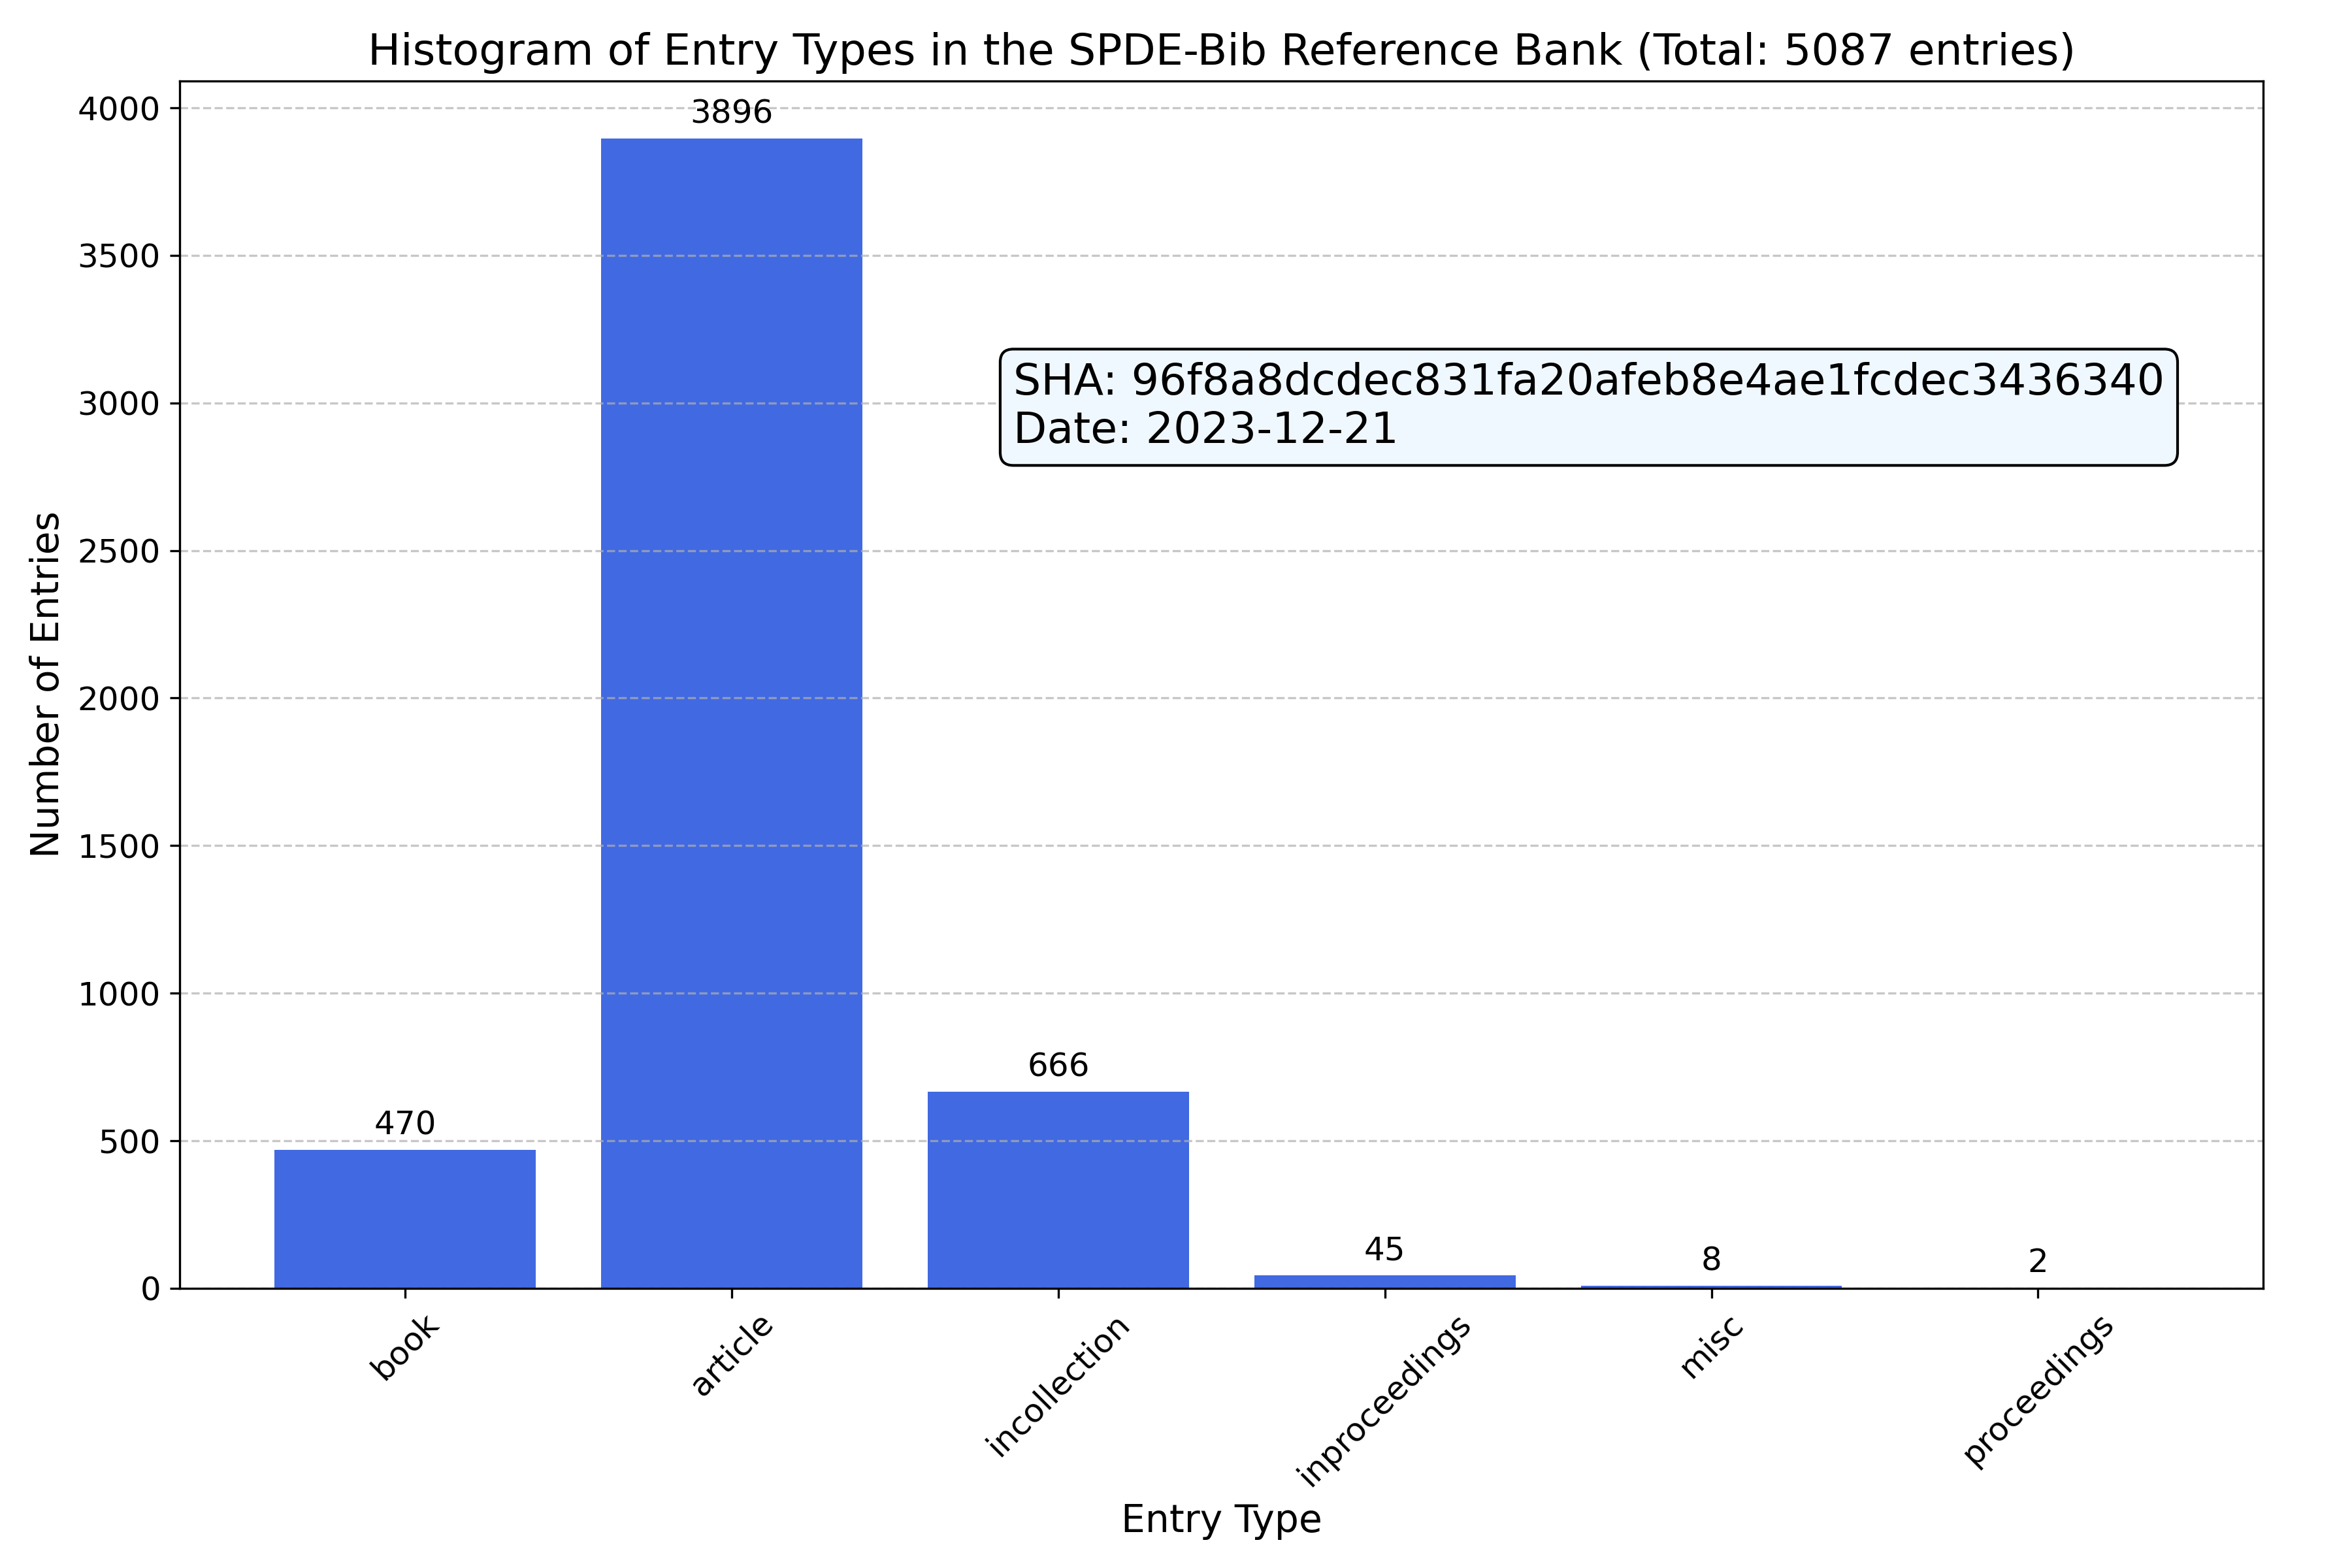
\includegraphics[scale=0.55]{Statistics.png}
\end{center}


\newpage
\tableofcontents

\newpage

\section{Introduction}

\subsection{Motivation}

When writing a paper, it is not an easy task to keep the bibliography part
correct and updated. This process is also very time-consuming. Through this
repo, we provide a uniform access to the latest bibliography entries related to
the research area of the author: \textit{Stochastic Partial Differential
Equations} (SPDEs) and related fields.


\subsection{Sources}
Here is a reference bank. The biblatex entries were mostly obtained from

\begin{center}
  \url{https://mathscinet.ams.org/mathscinet}
\end{center}

\noindent for the published mathematics papers and from the \textit{arXiv} for
the preprint. Some physics papers are obtained from
\begin{center}
  \url{https://journals.aps.org/search/}
\end{center}


\noindent For papers that do not originate from the aforementioned sources, we
endeavor to retrieve the bibliography entry directly from the official journal
website to ensure maximum accuracy of the records.


\subsection{Naming convention}

The naming convention consists of three cases:
\begin{enumerate}
  \item Single authored paper, such as:
  \item[] Einstein, Albert. Random PDE for special relativities.
    \textit{Annals of Probability}, Volume, Number, 2023.
    \begin{center}
      einstein:23:random
    \end{center}
    \bigskip

  \item Paper with two authors, such as:
  \item[] Einstein, Albert and Grothendieck, Alexandre. A stochastic PDE
    model for general relativities. \textit{Electronic Journal of Probability},
    Volume, Number, 2024.
    \begin{center}
      einstein.grothendieck:24:stochastic
    \end{center}

  \item Paper with more than two authors, such as:
  \item[] Einstein, Albert and Grothendieck, Alexandre and Newton, Isaac.
    A private communication on interemittency. \textit{Transactions of AMS},
    Volume, Number, 2025.
    \begin{center}
      einstein.grothendieck.ea:25:private
    \end{center}
\end{enumerate}
\bigskip

Here is a demonstration how to use it in neovim:
\begin{center}
  \url{https://asciinema.org/a/596819}.
\end{center}

\subsection{How to contribute}

We strive for accuracy and comprehensiveness in this bibliography bank. If you
encounter any errors, typos, or issues, or if you would like to suggest
additional entries, we warmly welcome your input. Your contributions are
invaluable to the enhancement of this resource. Please feel free to open an
issue in the repository or reach out directly via email
(\url{chenle02@gmail.com}) for any such matters. We aim to address all feedback
promptly.

\subsection{Acknowledgments}

We hope that the resources compiled in this bibliography bank have been
supportive in your research endeavors. We are sincerely grateful for any form of
acknowledgment you might extend. Should you wish to mention this work, a
statement such as the one below could be included in your acknowledgments
section or as a footnote:

\begin{quotation}
  The author(s) would like to recognize the contribution of the GitHub
  repository chenle02/SPDEs-Bib curated by Le Chen, which has supported this
  research.
\end{quotation}

Or, if you prefer to directly cite this repository, please feel free
to use the following BibTeX entry:

\begin{verbatim}
@misc{chen:22:spdes-bib,
  author       = {Chen, Le},
  title        = {SPDEs-Bib: A Comprehensive Bibliography of
                  Stochastic Partial Differential Equations
                  and Related Topics},
  year         = {2022},
  publisher    = {GitHub Repository},
  howpublished = {\url{https://github.com/chenle02/SPDEs-Bib}},
  note         = {Accessed: 11/11/2023, V1.0},
}
\end{verbatim}

\newpage
\section{All references listed by the citation keys}

\citeall

\newpage
\newgeometry{margin=1in, left=2.5in}

\section{All references}

\subsection{Articles}%
\label{sec:Articles}

\printbibliography[type=article,title={Articles}]
\subsection{Books}%
\label{ssec:Books}

\printbibliography[type=book,title={Books}]

\subsection{In proceedings}%
\label{ssec:In proceedings}

\printbibliography[type=inproceedings,title={In proceedings}]

\subsection{In collections}%
\label{ssec:In collections}

\printbibliography[type=incollection,title={In collection}]

\end{document}
